% Options for packages loaded elsewhere
\PassOptionsToPackage{unicode}{hyperref}
\PassOptionsToPackage{hyphens}{url}
%
\documentclass[
]{book}
\usepackage{lmodern}
\usepackage{amssymb,amsmath}
\usepackage{ifxetex,ifluatex}
\ifnum 0\ifxetex 1\fi\ifluatex 1\fi=0 % if pdftex
  \usepackage[T1]{fontenc}
  \usepackage[utf8]{inputenc}
  \usepackage{textcomp} % provide euro and other symbols
\else % if luatex or xetex
  \usepackage{unicode-math}
  \defaultfontfeatures{Scale=MatchLowercase}
  \defaultfontfeatures[\rmfamily]{Ligatures=TeX,Scale=1}
\fi
% Use upquote if available, for straight quotes in verbatim environments
\IfFileExists{upquote.sty}{\usepackage{upquote}}{}
\IfFileExists{microtype.sty}{% use microtype if available
  \usepackage[]{microtype}
  \UseMicrotypeSet[protrusion]{basicmath} % disable protrusion for tt fonts
}{}
\makeatletter
\@ifundefined{KOMAClassName}{% if non-KOMA class
  \IfFileExists{parskip.sty}{%
    \usepackage{parskip}
  }{% else
    \setlength{\parindent}{0pt}
    \setlength{\parskip}{6pt plus 2pt minus 1pt}}
}{% if KOMA class
  \KOMAoptions{parskip=half}}
\makeatother
\usepackage{xcolor}
\IfFileExists{xurl.sty}{\usepackage{xurl}}{} % add URL line breaks if available
\IfFileExists{bookmark.sty}{\usepackage{bookmark}}{\usepackage{hyperref}}
\hypersetup{
  pdftitle={Engagement Survey Technical Report},
  pdfauthor={Eagle I.O},
  hidelinks,
  pdfcreator={LaTeX via pandoc}}
\urlstyle{same} % disable monospaced font for URLs
\usepackage{longtable,booktabs}
% Correct order of tables after \paragraph or \subparagraph
\usepackage{etoolbox}
\makeatletter
\patchcmd\longtable{\par}{\if@noskipsec\mbox{}\fi\par}{}{}
\makeatother
% Allow footnotes in longtable head/foot
\IfFileExists{footnotehyper.sty}{\usepackage{footnotehyper}}{\usepackage{footnote}}
\makesavenoteenv{longtable}
\usepackage{graphicx,grffile}
\makeatletter
\def\maxwidth{\ifdim\Gin@nat@width>\linewidth\linewidth\else\Gin@nat@width\fi}
\def\maxheight{\ifdim\Gin@nat@height>\textheight\textheight\else\Gin@nat@height\fi}
\makeatother
% Scale images if necessary, so that they will not overflow the page
% margins by default, and it is still possible to overwrite the defaults
% using explicit options in \includegraphics[width, height, ...]{}
\setkeys{Gin}{width=\maxwidth,height=\maxheight,keepaspectratio}
% Set default figure placement to htbp
\makeatletter
\def\fps@figure{htbp}
\makeatother
\setlength{\emergencystretch}{3em} % prevent overfull lines
\providecommand{\tightlist}{%
  \setlength{\itemsep}{0pt}\setlength{\parskip}{0pt}}
\setcounter{secnumdepth}{5}
\usepackage{booktabs}
\usepackage[]{natbib}
\bibliographystyle{plainnat}

\title{Engagement Survey Technical Report}
\author{Eagle I.O}
\date{Most recently updated 2020-11-05}

\begin{document}
\maketitle

{
\setcounter{tocdepth}{4}
\tableofcontents
}
\hypertarget{homepage}{%
\chapter{Home}\label{homepage}}


\includegraphics{EE.jpeg}

This is a report that documents the technical details regarding the development of the Eagle I.O Engagement survey.

\hypertarget{intro}{%
\chapter{Introduction}\label{intro}}


\includegraphics{research.jpg}

Work engagement is the mental state where employees\ldots{}

\begin{itemize}
\tightlist
\item
  \ldots feel full with physical energy (\textbf{Vigor})
\item
  \ldots are enthusiastic about the content of their work and the things they do (\textbf{Dedication})
\item
  \ldots are so immersed in their work activities that time seems to fly (\textbf{Absorption})
\end{itemize}

These above definitions come from \citet{bakker_job_2017}.

The tripartite substantive model of employee engagement is also partially informed by the definitions provided with the Utrecht Work Engagement Scale \citep{schaufeli_utrecht_2003}.

We lost the document where we had saved the citations for the creation of our engagement dimensions. we found it today (02/04/2020).
Three out of the four dimensions (Dedication, Vigor, and Absorbtion) came from \citet{schaufeli_measurement_2002}, and we are trying to find where Fulfillment came from.
We are also trying to improve the definition of each domain by looking at the current items and conducting a Modified Q sort (not correct name) to create piles of items that have commonalities within each domain.

\hypertarget{ABCDAV}{%
\section{Intended Structure}\label{ABCDAV}}

At some point we decided to attempt an \emph{a priori} bi-factor structure, whereby each of the substantive dimensions (Dedication, Vigor, and Absorption)\footnote{We also discovered at this point that some contagious agent has infiltrated the minds of people working on this project, such that the word, ``absorption'' confounds our spelling abilities, and roughly 50\% of the time ends up being spelled (misspelled?), ``absorbtion''\ldots{}} could further be deconstructed into the attitudinal elements of Cognition, Affect, and Behavior. Through item-writing and revision, it began to dawn on us that the substantive elements may already reflect the Cognition (Vigor), Affect (Absorption), and Behavioral (Dedication) dimensions.

As of August, 2012, we could not locate a source article that made this alignment explicit, so we persisted through crafting items that reflected Cognitive, Affective, and Behavioral indicators of each substantive dimension.

The most relevant acknowledgement of this potential confound was made by \citet{schaufeli_measurement_2002} (p.~??):

\begin{quote}
Hence, engagement is defined as a positive, fulfilling, work-related state of mind that is characterized by vigor, dedication, and absorption. Rather than a momentary and specific state, engagement refers to a more persistent and pervasive affective cognitive state that is not focused on any particular object, event, individual, or behavior. Vigor is characterized by high levels of energy and mental resilience while working, the willingness to invest effort in one's work, and persistence even in the face of difficulties. Dedication is characterized by a sense of significance, enthusiasm, inspiration, pride, and challenge. Instead of involvement we prefer to use the term dedication. Although, involvement -- like dedication (see above) -- is usually defined in terms of psychological identification with one's work or one's job (Kanungo, 1982; Lawler and Hall, 1970), whereby the latter goes one step beyond, both quantitatively as well as qualitatively. In a qualitative sense, dedication refers to a particularly strong involvement that goes one step further than the usual level of identification.
\end{quote}

The survey is intentionally complex in terms of item and scale associations. There are three substantive engagement dimensions as well as three attitudinal dimensions, and item cross-loadings are intended to fully exhaust the 3 x 3 conditions (e.g., each item loads on one substantive and one attitudinal dimension):

\begin{longtable}[]{@{}ll@{}}
\toprule
Substantive & Attitudinal\tabularnewline
\midrule
\endhead
Dedication & Affective\tabularnewline
Absorption & Behavioral\tabularnewline
Vigor & Cognitive\tabularnewline
\bottomrule
\end{longtable}

The feedback report uses the terms, ``feel'', ``do'', and ``think'' instead of the Psychological literature-based affect, behavior, and cognition \citep[see, for example,][]{eagly_psychology_1993}.

\hypertarget{instrument-creation}{%
\chapter{Instrument creation}\label{instrument-creation}}


\includegraphics{develop.jpg}

\hypertarget{item-generation}{%
\section{Item generation}\label{item-generation}}

After content validation but prior to settling on 4 candidate items per 3x3 condition, there was a dearth of items within some of the Affective, Cognitive, or Behavioral item groupings. We generated additional candidates at this point and have these items \href{https://docs.google.com/document/d/1whB4Ve4aDDl3bxx3dIlloouTDy1ScCcxrT3gK6s9DyU/edit?usp=sharing}{located here} (Montclair State University e-mail needed to access). It was from this larger list of (reduced) candidate items that the 36 pilot candidates were identified (and in some cases modified, edited, or otherwise further crafted)

\hypertarget{content-validation}{%
\section{Content Validation}\label{content-validation}}

7 Eagle I.O consultants were twice instructed to place each of 34 items into one of three categories: Absorption, Dedication, or Vigor, and Cognitive, Affective, or Behavioral. Instructions asked each rater to:

\begin{quote}
INSTRUCTIONS: Place an ``X'' in the column that you feel is the best fit for each item (only one ``X'' per row please)
\end{quote}

\hypertarget{administration-condition}{%
\section{Administration condition}\label{administration-condition}}

In order to randomize the administration of conditions, we asked respondents to indicate their birth month:

\begin{itemize}
\tightlist
\item
  January \(\rightarrow\) March: LINK ONE
\item
  April \(\rightarrow\) June: LINK TWO
\item
  July \(\rightarrow\) September: LINK THREE
\item
  October \(\rightarrow\) December: LINK FOUR
\end{itemize}

The substantive scale definitions provided for ratings were:

\begin{itemize}
\tightlist
\item
  \emph{Absorption}: Being fully immersed in one's work, where time passes quickly and one has difficulty detaching from work tasks
\item
  \emph{Vigor}: Experiencing persistent levels of energy, effort, and enthusiasm while working
\item
  \emph{Dedication}: Experiencing pride and challenge in ones work, as well as strong feelings of support from and loyalty toward the organization
\end{itemize}

The attitudinal scale definitions were:

\begin{itemize}
\tightlist
\item
  \emph{Cognitive}: Pertaining to thoughts or general mental processes (for example what someone thinks)
\item
  \emph{Affective}: Pertaining to feelings or emotions (for example, how someone feels)
\item
  \emph{Behavioral}: Pertaining to acts or actions (for example, what someone does)
\end{itemize}

The goal was to identify item(s) that were equally and heavily implicated with one substantive and one attitudinal scale.

Initial rating convergence for Absorption:

\begin{verbatim}
##           Cognitive
## Absorption 1 2 4 5 6 7
##          1 2 1 0 1 0 0
##          2 0 0 0 0 0 0
##          4 1 1 0 0 0 0
##          5 0 1 0 0 0 0
##          6 0 0 0 0 0 0
##          7 0 2 0 0 0 0
\end{verbatim}

\begin{verbatim}
##           Affective
## Absorption 1 2 3 4 5 6 7
##          1 0 1 0 0 1 1 0
##          2 0 0 0 0 0 0 0
##          4 0 0 0 0 1 0 0
##          5 0 0 0 0 0 0 0
##          6 0 0 0 0 0 0 0
##          7 0 2 0 0 0 0 0
\end{verbatim}

\begin{verbatim}
##           Behavioral
## Absorption 1 2 3 5 6 7
##          1 1 0 0 1 0 0
##          2 0 0 0 0 0 1
##          4 0 0 0 0 2 0
##          5 0 0 0 1 1 0
##          6 0 0 0 0 0 1
##          7 0 0 2 0 0 1
\end{verbatim}

Initial rating convergence for Vigor:

\begin{verbatim}
##      Cognitive
## Vigor 1 2 4 5 6 7
##     1 0 0 1 0 0 1
##     2 1 1 0 0 0 0
##     3 0 1 0 1 0 0
##     5 0 0 0 0 0 0
##     6 2 1 0 0 0 0
##     7 2 0 0 0 0 0
\end{verbatim}

\begin{verbatim}
##      Affective
## Vigor 1 2 3 4 5 6 7
##     1 0 0 1 0 0 0 0
##     2 0 0 0 0 0 0 0
##     3 0 1 0 0 1 0 0
##     5 0 0 0 0 0 1 0
##     6 0 0 0 0 1 1 1
##     7 0 0 0 1 0 3 1
\end{verbatim}

\begin{verbatim}
##      Behavioral
## Vigor 1 2 3 5 6 7
##     1 0 0 0 0 1 1
##     2 0 0 0 1 1 0
##     3 0 0 0 0 1 0
##     5 1 0 0 0 0 1
##     6 1 0 0 1 0 0
##     7 2 1 0 0 0 1
\end{verbatim}

Initial rating convergence for Dedication:

\begin{verbatim}
##           Cognitive
## Dedication 1 2 4 5 6 7
##          1 1 0 0 0 0 0
##          2 0 0 0 0 0 0
##          3 0 0 0 1 0 0
##          6 0 0 1 0 0 1
##          7 0 2 0 4 1 1
\end{verbatim}

\begin{verbatim}
##           Affective
## Dedication 1 2 3 4 5 6 7
##          1 0 0 0 0 0 0 1
##          2 0 0 0 0 0 1 0
##          3 0 1 0 0 0 0 0
##          6 0 0 1 0 0 0 0
##          7 1 3 0 0 1 0 1
\end{verbatim}

\begin{verbatim}
##           Behavioral
## Dedication 1 2 3 5 6 7
##          1 0 0 0 0 2 0
##          2 1 0 0 0 0 0
##          3 0 0 0 0 0 0
##          6 0 0 0 0 0 0
##          7 1 2 0 2 0 0
\end{verbatim}

\hypertarget{results}{%
\chapter{Results}\label{results}}

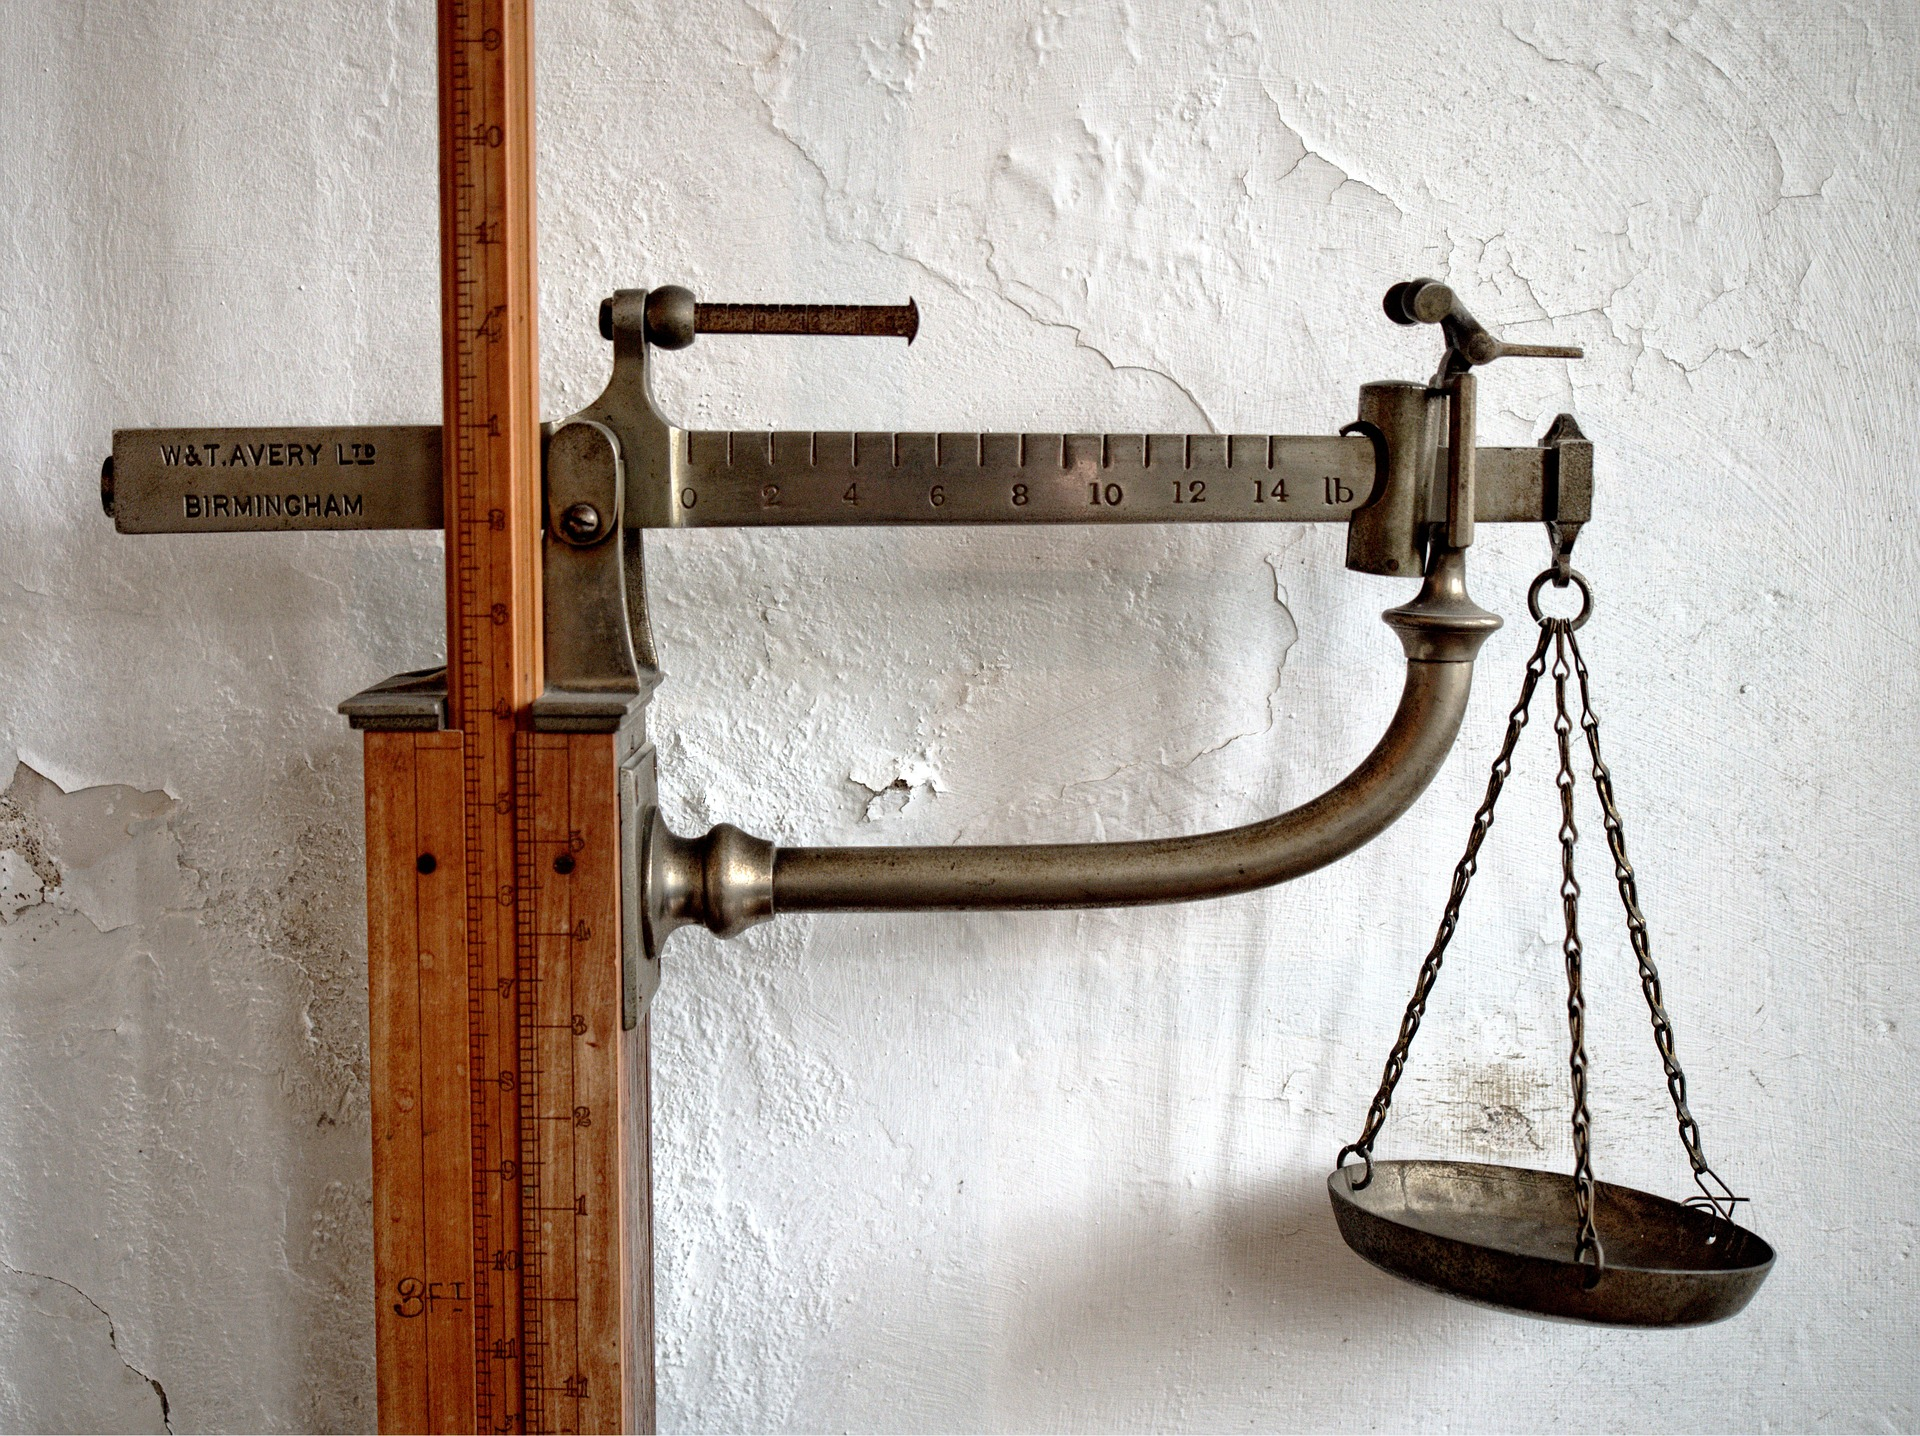
\includegraphics{results.jpg}

\hypertarget{pilot}{%
\section{Pilot}\label{pilot}}

The pilot administrations consisted of 36 \href{https://docs.google.com/document/d/18KYE7jq8XLhN-mfGQRMnkf5AM-_U2CJck50eISbAiwM/edit?usp=sharing}{items} that were presented in one of four administration groupings (see Appendix \ref{pilot2}): 1) within substantive dimension (attitudinally grouped {[}but randomized within blocks of 4{]}), 2) within attitudinal dimension (substantively grouped {[}but randomized within blocks of 4{]}), 3) within substantive dimension (randomly distributed by attitude), and 4) within attitudinal dimension (randomly presented by substance).\footnote{Decision was made on 10/13 to have the order of presentation \emph{randomized} within each of the broader organization blocks (for example, Condition 3: all Affective, Cognitive, and Behavioral Absorption items were randomly administered, then all ABC Dedication items, etc {[}although DAC was also randomized by block such that not every respondent had the same DAC ordering{]})}

The four ``experimental'' conditions therefore prioritized and reflected the 3x3 groupings \emph{or} one of the organization schemes (cognitive, affective, and behavioral \emph{or} dedication, absorption, and vigor).

We chose to control the order of item administration because of our \emph{a priori} specification of a bi-factor structure, with the expectation that item ordering would serve as a response cue, yeilding stronger factor structural support based on the organization scheme.

\hypertarget{sampling-strategy-pilot}{%
\subsection{Sampling strategy (pilot)}\label{sampling-strategy-pilot}}

Snowball sampling to reduce final instrument from 36 candidate items (4 per ``cell'').

Sampling plan (aim for 250 total responses):

\begin{itemize}
\tightlist
\item
  Eagle I.O members reach out via e-mail - draft e-mail that asks to forward along.
\item
  facebook post (MSU I.O)
\item
  LinkedIn (put on next agenda)
\item
  first-year students (Paulina posts in group-chat)

  \begin{itemize}
  \tightlist
  \item
    mentors also mention to mentees
  \item
    contact lists from Catrina
  \end{itemize}
\end{itemize}

\hypertarget{demographic-information}{%
\section{Demographic Information}\label{demographic-information}}

These are to be included in future administrations in an attempt to develop marketable norms:

\begin{itemize}
\tightlist
\item
  employees who work overtime vs.~those who do not
\item
  employees who get paid for overtime vs.~those who don't receive compensation for extra hours worked\footnote{I was thinking about this because at my job I have been working 12+ hours some days yet I do not get overtime pay. Not sure if this would work for what we are doing and I know my work experiences are not universal (nor should they be) haha!}
\end{itemize}

\hypertarget{construct-and-criterion-related-validation}{%
\section{Construct and Criterion-related Validation}\label{construct-and-criterion-related-validation}}

Use Gallup for construct validation \citep{thackray_gallup_2005}. Also the Utrecht Work Engagement Scale \citep[UWES;][]{schaufeli_measurement_2002, schaufeli_defining_2010}

\hypertarget{future-plans}{%
\chapter{Future plans}\label{future-plans}}


\includegraphics{future.jpg}

Development of the feedback report will occur in stages:

\begin{enumerate}
\def\labelenumi{\arabic{enumi}.}
\tightlist
\item
  Static .pdf
\item
  Dynamic dashboard
\item
  Optimize interpretation (invite contributions of cognitive psychologists and/or graphic designers)
\end{enumerate}

\hypertarget{things-to-do}{%
\section{Things to do}\label{things-to-do}}

\begin{itemize}
\tightlist
\item
  Finalize items
\item
  Get survey into Qualtrics for pilot testing
\item
  Work on feedback report
\end{itemize}

\hypertarget{author-bios}{%
\chapter{Author bios}\label{author-bios}}


\includegraphics{casey.jpg}

\href{mailto:osorioduffc1@montclair.edu}{Casey Osorio-Duffoo}

\href{mailto:garciaprier1@mail.montclair.edu}{Renata Garcia Prieto Palacios Roji} received her BA in Psychology and minor in Philosophy from the University of Texas in 2017. Her I/O interests include Data analysis, Learning and Development, and Executive coaching.


\includegraphics{renata.jpg}


\includegraphics{kulas.jpg}

\href{mailto:kulasj@montclair.edu}{John Kulas}

\hypertarget{references}{%
\chapter{References}\label{references}}

\citet{eagly_psychology_1993}
\citeauthor{simpson_engagement_2009} \citetext{\citeyear{simpson_engagement_2009}; \citealp{harter_business_2002}; \citealp{kahn_psychological_1990}; \citealp{leiter_areas_2003}; \citealp{R-base}; \citealp{R-rmarkdown}; \citealp{rothbard_enriching_2001}; \citealp{saks_antecedents_2006}; \citealp{schaufeli_measurement_2002}; \citealp{simpson_engagement_2009}}

\hypertarget{refs}{}

\hypertarget{appendix-appendices}{%
\appendix}


\hypertarget{timeline-of-events}{%
\chapter{Timeline of events}\label{timeline-of-events}}

Here is Eagle IO's initial definition of engagement (Spring 2019):

A state of personal immersion in work characterized by enthusiasm, dedication, and personal investment, expressed cognitively, affectively, and behaviorally in the proactive pursuit of advancing organizational goals.

This definition was created by Eagle IO Spring 2019, and modified by Dr.~Kulas and Renata Fall 2019 to include the four dimensions of Fulfillment, Absorbtion, Dedication, and Vigor.

\hypertarget{feb-20.2020-considering-removing-fulfillment}{%
\section{Feb 20.2020 (Considering removing fulfillment)}\label{feb-20.2020-considering-removing-fulfillment}}

\emph{Fulfillment}: finding meaning in one's work, while having a sense of autonomy, growth, usefulness, achievement, and feeling appreciated by org. {[}Satisfaction(?){]}

Decided to operationalize fullfillment as an \emph{outcome} of engagement rather than a definitional element

\hypertarget{definitional-amendments-as-of-02.24.2020}{%
\section{Definitional amendments as of 02.24.2020}\label{definitional-amendments-as-of-02.24.2020}}

\emph{Absorption}: being fully concentrated and happily immersed in ones work (time passes quickly and has difficulty detaching from ones work; Schaufeli et al., 2002)

\emph{Dedication/Commitment}: being strongly involved in one's work and experiencing a sense of enthusiasm, inspiration, pride, and challenge. (Schaufeli et al., 2002) Identifying as an organizational member/ambassador

include identification with the organization, a sense of ``oneness''
seeking continuous leanring and improvement
getting rid of challenge altogether
moving inspiration and pride to other categories

\emph{dedication}: seeking continous imporvement and demonstrating initiative

\emph{Vigor}: investing consistent effort, persistence, energy, and mental resilience while working (Schaufeli et al., 2002)
maybe add enthusiasm here as well

\emph{Vigor}: Experiencing persistent levels of energy and enthusiasm while working

\begin{center}\rule{0.5\linewidth}{0.5pt}\end{center}

potential to change from affective, cognitive, and behavioral to whether their engagement comes from content/satisfaction with the organization or the people they work with.

\begin{center}\rule{0.5\linewidth}{0.5pt}\end{center}

After completing individual Q-sorts (Kulas and Renata) we decided to revisit the definitions and build them up a little to make the difference between them more noticeable.

\hypertarget{definitions-as-of-5192020}{%
\section{Definitions as of 5/19/2020}\label{definitions-as-of-5192020}}

\emph{Absorption}: Being fully immersed in one's work, where time passes quickly and one has difficulty detaching from work tasks

\emph{Vigor}: Experiencing persistent levels of energy, effort, and enthusiasm while working

\emph{Dedication}: Experiencing pride and challenge in ones work, as well as strong feelings of support from and loyalty toward the organization

With these definitions we ordered all the items according to the ones we individually selected for each category and created an item bank with the remaining items. Together we placed the items in the bank into the agreed upon categories.

\hypertarget{pilot2}{%
\chapter{Pilot conditions}\label{pilot2}}

Our four orderings of items were randomized within dimension (Affective, Behavioral, Cognitive or Dedication, Absorption, Vigor), ``block'' (Qualtrics designation for groupings of items), and item. The elements that were randomized are identified in the following tables by randomized element (A, B, C, or D):

\label{tab:conditions}Pilot administration ordering Condition 1

Condition1

Substantive

Attitudinal

Dimension

Block

Item

I'm able to concentrate on my work without distractions

Absorption

Cognitive

A

A

A

I have a hard time detaching mentally from my work

Absorption

Cognitive

A

A

B

Time passes quickly while I'm working

Absorption

Cognitive

A

A

C

I find it difficult to mentally disconnect from work

Absorption

Cognitive

A

A

D

I enjoy thinking about work even when I'm not at work

Absorption

Affective

A

B

A

Most days, I feel happiest when the workday is soon to be complete (r)

Absorption

Affective

A

B

B

I am happiest when I am immersed in a project

Absorption

Affective

A

B

C

I love starting my workday.

Absorption

Affective

A

B

D

I devote more time than is expected of me.

Absorption

Behavioral

A

C

A

I have to be reminded to take breaks while I'm at work

Absorption

Behavioral

A

C

B

I never miss a work deadline.

Absorption

Behavioral

A

C

C

I never allow distractions to interfere with my work

Absorption

Behavioral

A

C

D

I devote my full attention to my work tasks throughout the day

Vigor

Cognitive

B

A

A

Thinking about work saps my energy (r)

Vigor

Cognitive

B

A

B

I would rather direct my focus toward a work task than a personal task

Vigor

Cognitive

B

A

C

I'm able to maintain good levels of energy throughout the workday

Vigor

Cognitive

B

A

D

I enjoy spending time completing my job tasks.

Vigor

Affective

B

B

A

Most days I feel enthusiastic about starting my work day.

Vigor

Affective

B

B

B

I feel motivated to go beyond what is asked of me

Vigor

Affective

B

B

C

This job drains my energy (r)

Vigor

Affective

B

B

D

When work is slow I find ways to be productive.

Vigor

Behavioral

B

C

A

I express enthusiasm for my job while at work

Vigor

Behavioral

B

C

B

I try my best to perform well at work

Vigor

Behavioral

B

C

C

If I notice my energy level is low, I take corrective steps to re-energize.

Vigor

Behavioral

B

C

D

I plan my future with this company.

Dedication

Cognitive

C

A

A

I believe this company cares about my career goals

Dedication

Cognitive

C

A

B

I often think about finding another job (r)

Dedication

Cognitive

C

A

C

This organization challenges me to work at my full potential

Dedication

Cognitive

C

A

D

I am proud to be a member of this organization.

Dedication

Affective

C

B

A

I feel supported by my supervisor when I fail at a task

Dedication

Affective

C

B

B

I feel proud of my accomplishments within this organization

Dedication

Affective

C

B

C

My job makes me feel like I'm part of something meaningful

Dedication

Affective

C

B

D

I make valued contributions to the organization

Dedication

Behavioral

C

C

A

I embrace challenging situations at work.

Dedication

Behavioral

C

C

B

I speak positively about this organization to others.

Dedication

Behavioral

C

C

C

This organization provides the resources necessary for me to successfully perform my job

Dedication

Behavioral

C

C

D

\label{tab:conditions}Pilot administration ordering Condition 2

Condition2

Substantive

Attitudinal

Dimension

Block

Item

I'm able to concentrate on my work without distractions

Absorption

Cognitive

A

A

A

I have a hard time detaching mentally from my work

Absorption

Cognitive

A

A

B

Time passes quickly while I'm working

Absorption

Cognitive

A

A

C

I find it difficult to mentally disconnect from work

Absorption

Cognitive

A

A

D

I devote my full attention to my work tasks throughout the day

Vigor

Cognitive

A

B

A

Thinking about work saps my energy (r)

Vigor

Cognitive

A

B

B

I would rather direct my focus toward a work task than a personal task

Vigor

Cognitive

A

B

C

I'm able to maintain good levels of energy throughout the workday

Vigor

Cognitive

A

B

D

I plan my future with this company.

Dedication

Cognitive

A

C

A

I believe this company cares about my career goals

Dedication

Cognitive

A

C

B

I often think about finding another job (r)

Dedication

Cognitive

A

C

C

This organization challenges me to work at my full potential

Dedication

Cognitive

A

C

D

I enjoy thinking about work even when I'm not at work

Absorption

Affective

B

A

A

Most days, I feel happiest when the workday is soon to be complete (r)

Absorption

Affective

B

A

B

I am happiest when I am immersed in a project

Absorption

Affective

B

A

C

I love starting my workday.

Absorption

Affective

B

A

D

I enjoy spending time completing my job tasks.

Vigor

Affective

B

B

A

Most days I feel enthusiastic about starting my work day.

Vigor

Affective

B

B

B

I feel motivated to go beyond what is asked of me

Vigor

Affective

B

B

C

This job drains my energy (r)

Vigor

Affective

B

B

D

I am proud to be a member of this organization.

Dedication

Affective

B

C

A

I feel supported by my supervisor when I fail at a task

Dedication

Affective

B

C

B

I feel proud of my accomplishments within this organization

Dedication

Affective

B

C

C

My job makes me feel like I'm part of something meaningful

Dedication

Affective

B

C

D

I devote more time than is expected of me.

Absorption

Behavioral

C

A

A

I have to be reminded to take breaks while I'm at work

Absorption

Behavioral

C

A

B

I never miss a work deadline.

Absorption

Behavioral

C

A

C

I never allow distractions to interfere with my work

Absorption

Behavioral

C

A

D

When work is slow I find ways to be productive.

Vigor

Behavioral

C

B

A

I express enthusiasm for my job while at work

Vigor

Behavioral

C

B

B

I try my best to perform well at work

Vigor

Behavioral

C

B

C

If I notice my energy level is low, I take corrective steps to re-energize.

Vigor

Behavioral

C

B

D

I make valued contributions to the organization

Dedication

Behavioral

C

C

A

I embrace challenging situations at work.

Dedication

Behavioral

C

C

B

I speak positively about this organization to others.

Dedication

Behavioral

C

C

C

This organization provides the resources necessary for me to successfully perform my job

Dedication

Behavioral

C

C

D

\label{tab:conditions}Pilot administration ordering Condition 3

Condition3

Substantive

Attitudinal

Dimension

Item

I'm able to concentrate on my work without distractions

Absorption

Cognitive

A

A

I enjoy thinking about work even when I'm not at work

Absorption

Affective

A

B

I devote more time than is expected of me.

Absorption

Behavioral

A

C

I have a hard time detaching mentally from my work

Absorption

Cognitive

A

D

Most days, I feel happiest when the workday is soon to be complete (r)

Absorption

Affective

A

E

I have to be reminded to take breaks while I'm at work

Absorption

Behavioral

A

F

Time passes quickly while I'm working

Absorption

Cognitive

A

G

I am happiest when I am immersed in a project

Absorption

Affective

A

H

I never miss a work deadline.

Absorption

Behavioral

A

I

I find it difficult to mentally disconnect from work

Absorption

Cognitive

A

J

I love starting my workday.

Absorption

Affective

A

K

I never allow distractions to interfere with my work

Absorption

Behavioral

A

L

I devote my full attention to my work tasks throughout the day

Vigor

Cognitive

B

A

I enjoy spending time completing my job tasks.

Vigor

Affective

B

B

When work is slow I find ways to be productive.

Vigor

Behavioral

B

C

Thinking about work saps my energy (r)

Vigor

Cognitive

B

D

Most days I feel enthusiastic about starting my work day.

Vigor

Affective

B

E

I express enthusiasm for my job while at work

Vigor

Behavioral

B

F

I would rather direct my focus toward a work task than a personal task

Vigor

Cognitive

B

G

I feel motivated to go beyond what is asked of me

Vigor

Affective

B

H

I try my best to perform well at work

Vigor

Behavioral

B

I

I'm able to maintain good levels of energy throughout the workday

Vigor

Cognitive

B

J

This job drains my energy (r)

Vigor

Affective

B

K

If I notice my energy level is low, I take corrective steps to re-energize.

Vigor

Behavioral

B

L

I plan my future with this company.

Dedication

Cognitive

C

A

I am proud to be a member of this organization.

Dedication

Affective

C

B

I make valued contributions to the organization

Dedication

Behavioral

C

C

I believe this company cares about my career goals

Dedication

Cognitive

C

D

I feel supported by my supervisor when I fail at a task

Dedication

Affective

C

E

I embrace challenging situations at work.

Dedication

Behavioral

C

F

I often think about finding another job (r)

Dedication

Cognitive

C

G

I feel proud of my accomplishments within this organization

Dedication

Affective

C

H

I speak positively about this organization to others.

Dedication

Behavioral

C

I

This organization challenges me to work at my full potential

Dedication

Cognitive

C

J

My job makes me feel like I'm part of something meaningful

Dedication

Affective

C

K

This organization provides the resources necessary for me to successfully perform my job

Dedication

Behavioral

C

L

\label{tab:conditions}Pilot administration ordering Condition 4

Condition4

Substantive

Attitudinal

Dimension

Item

I'm able to concentrate on my work without distractions

Absorption

Cognitive

A

A

I devote my full attention to my work tasks throughout the day

Vigor

Cognitive

A

B

I plan my future with this company.

Dedication

Cognitive

A

C

I have a hard time detaching mentally from my work

Absorption

Cognitive

A

D

Thinking about work saps my energy (r)

Vigor

Cognitive

A

E

I believe this company cares about my career goals

Dedication

Cognitive

A

F

Time passes quickly while I'm working

Absorption

Cognitive

A

G

I would rather direct my focus toward a work task than a personal task

Vigor

Cognitive

A

H

I often think about finding another job (r)

Dedication

Cognitive

A

I

I find it difficult to mentally disconnect from work

Absorption

Cognitive

A

J

I'm able to maintain good levels of energy throughout the workday

Vigor

Cognitive

A

K

This organization challenges me to work at my full potential

Dedication

Cognitive

A

L

I enjoy thinking about work even when I'm not at work

Absorption

Affective

B

A

I enjoy spending time completing my job tasks.

Vigor

Affective

B

B

I am proud to be a member of this organization.

Dedication

Affective

B

C

Most days, I feel happiest when the workday is soon to be complete (r)

Absorption

Affective

B

D

Most days I feel enthusiastic about starting my work day.

Vigor

Affective

B

E

I feel supported by my supervisor when I fail at a task

Dedication

Affective

B

F

I am happiest when I am immersed in a project

Absorption

Affective

B

G

I feel motivated to go beyond what is asked of me

Vigor

Affective

B

H

I feel proud of my accomplishments within this organization

Dedication

Affective

B

I

I love starting my workday.

Absorption

Affective

B

J

This job drains my energy (r)

Vigor

Affective

B

K

My job makes me feel like I'm part of something meaningful

Dedication

Affective

B

L

I devote more time than is expected of me.

Absorption

Behavioral

C

A

When work is slow I find ways to be productive.

Vigor

Behavioral

C

B

I make valued contributions to the organization

Dedication

Behavioral

C

C

I have to be reminded to take breaks while I'm at work

Absorption

Behavioral

C

D

I express enthusiasm for my job while at work

Vigor

Behavioral

C

E

I embrace challenging situations at work.

Dedication

Behavioral

C

F

I never miss a work deadline.

Absorption

Behavioral

C

G

I try my best to perform well at work

Vigor

Behavioral

C

H

I speak positively about this organization to others.

Dedication

Behavioral

C

I

I never allow distractions to interfere with my work

Absorption

Behavioral

C

J

If I notice my energy level is low, I take corrective steps to re-energize.

Vigor

Behavioral

C

K

This organization provides the resources necessary for me to successfully perform my job

Dedication

Behavioral

C

L

\hypertarget{qualitative-item-characteristics}{%
\chapter{Qualitative item characteristics}\label{qualitative-item-characteristics}}

Quentada reading ability of final items as well as overlapping histograms by scale. Using package \texttt{quanteda} in R version 4.0.2 (2020-06-22). The Flesch-Kincaid is the same grade level index that's currently used by Microsoft Word \citep{kincaid_derivation_1975}. ``Dale.Chall'' reflects \emph{N\textsubscript{wd}} \citep[``difficulty'' of words;][]{chall_dale_1995}. \href{https://quanteda.io/reference/textstat_readability.html}{\emph{N\textsubscript{wf}}} = the number of words matching the Dale-Chall List of 3000 ``familiar words''. \href{https://quanteda.io/reference/textstat_readability.html}{\emph{N\textsubscript{wd}}} = number of ``difficult'' words not matching the Dale-Chall list of ``familiar'' words.

The average Flesch-Kincaied (e.g., reading grade) was 6.2 (\emph{sd} = 3.04). The average Dale-Chall index was 38.61 (\emph{sd} = 11.11).

\hypertarget{frequency-distributions-by-dimension}{%
\section{Frequency distributions by dimension}\label{frequency-distributions-by-dimension}}

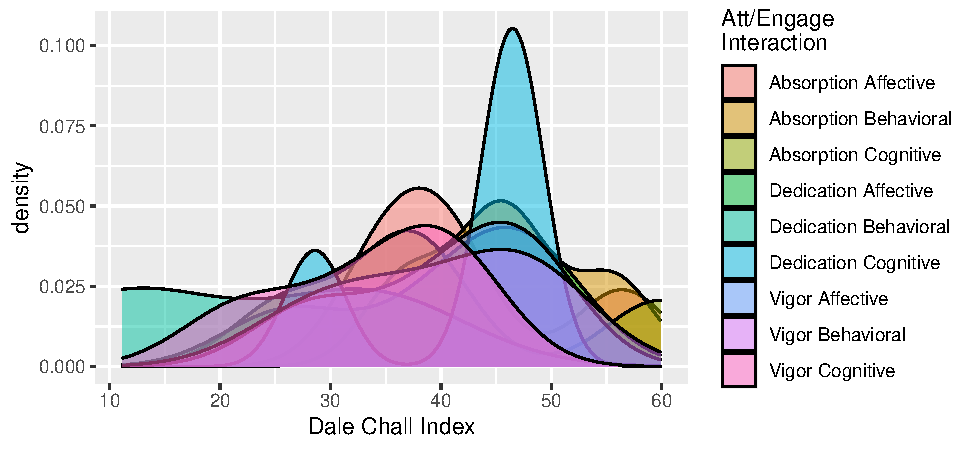
\includegraphics{_main_files/figure-latex/scale-1.pdf} 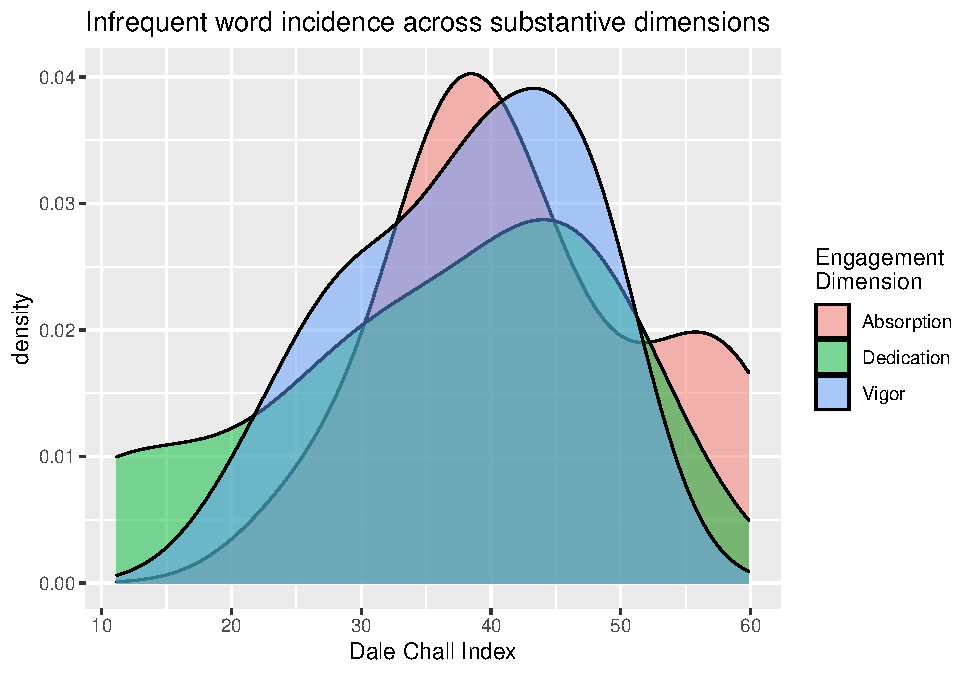
\includegraphics{_main_files/figure-latex/scale-2.pdf} 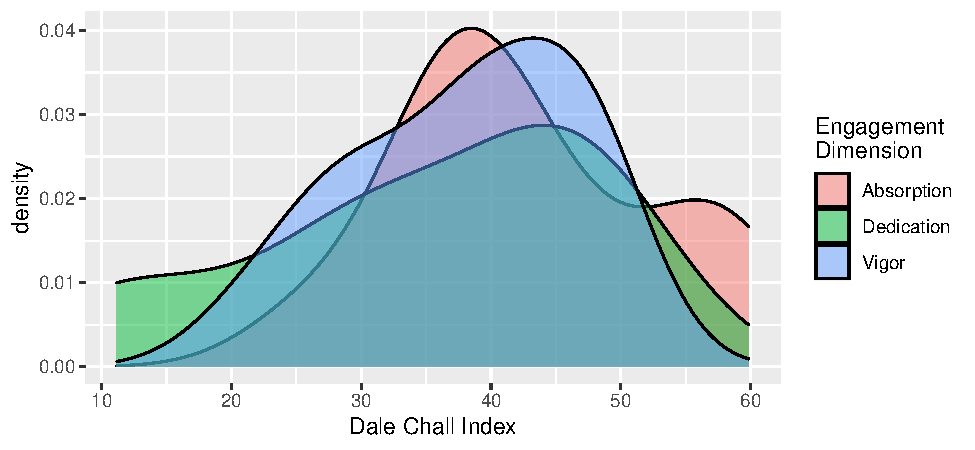
\includegraphics{_main_files/figure-latex/scale-3.pdf} 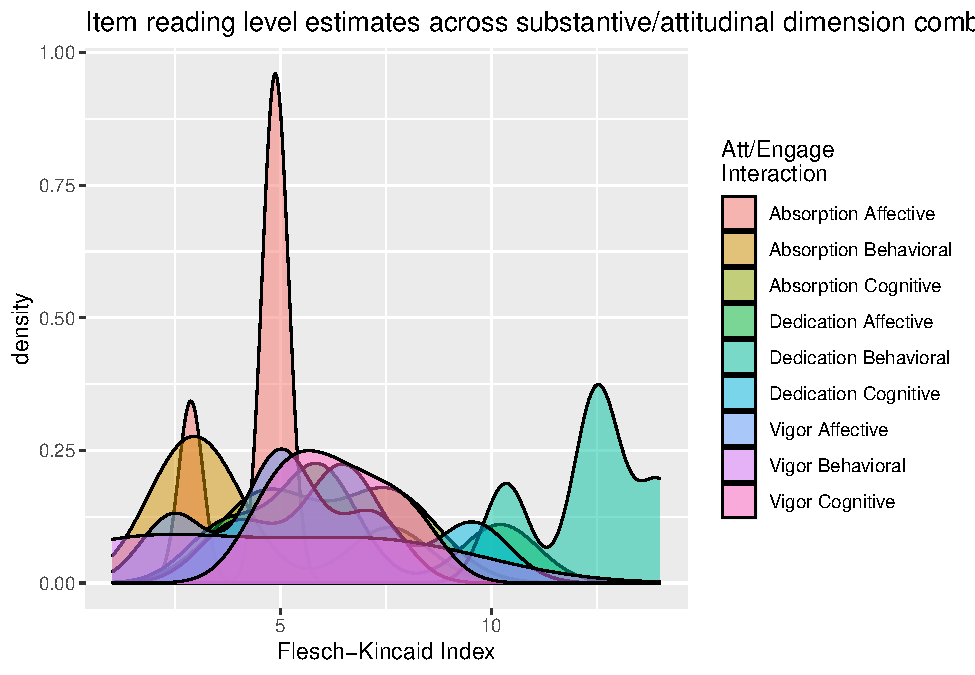
\includegraphics{_main_files/figure-latex/scale-4.pdf} 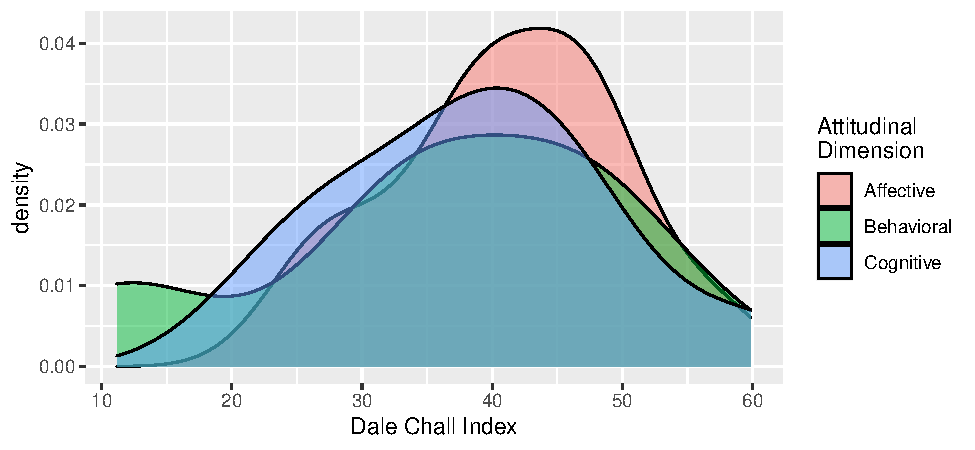
\includegraphics{_main_files/figure-latex/scale-5.pdf} 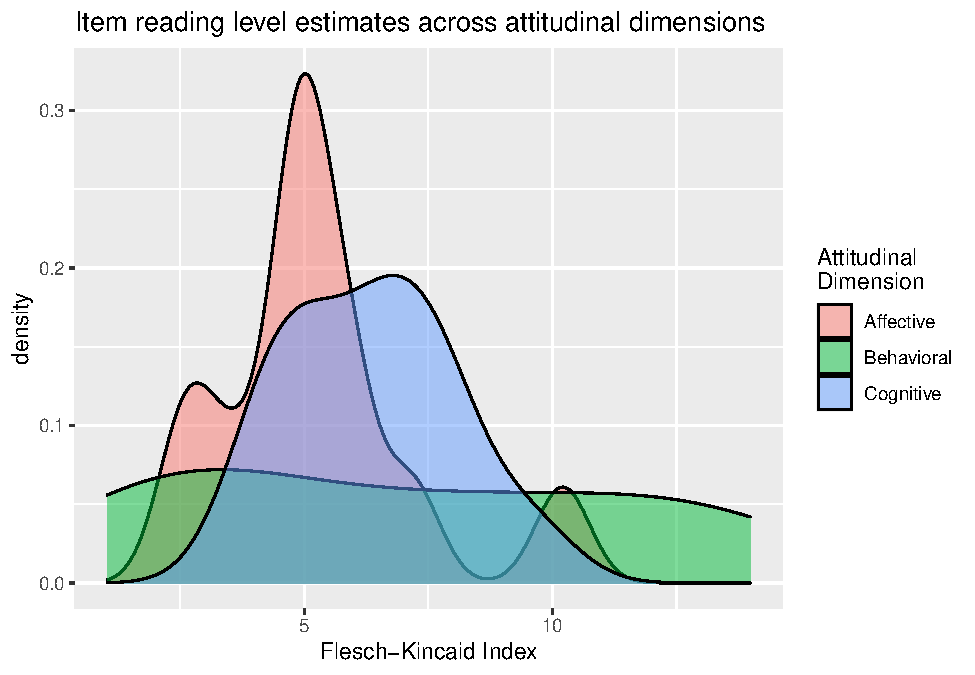
\includegraphics{_main_files/figure-latex/scale-6.pdf}

\hypertarget{tables-of-qualitative-indices}{%
\section{Tables of qualitative indices}\label{tables-of-qualitative-indices}}

\label{tab:freqtables}Organized by Flesch-Kincaid aka Reading Level

document

Substantive

Attitudinal

Flesch.Kincaid

Dale.Chall

36

This organization provides the resources necessary for me to successfully perform my job

Dedication

Behavioral

13.99

11.18

35

I speak positively about this organization to others.

Dedication

Behavioral

12.61

34.73

33

I make valued contributions to the organization

Dedication

Behavioral

12.43

32.03

34

I embrace challenging situations at work.

Dedication

Behavioral

10.35

12.36

31

I feel proud of my accomplishments within this organization

Dedication

Affective

10.21

26.12

28

This organization challenges me to work at my full potential

Dedication

Cognitive

9.55

28.60

24

If I notice my energy level is low, I take corrective steps to re-energize.

Vigor

Behavioral

8.35

28.32

16

I'm able to maintain good levels of energy throughout the workday

Vigor

Cognitive

8.01

21.86

1

I'm able to concentrate on my work without distractions

Absorption

Cognitive

7.59

36.68

4

I find it difficult to mentally disconnect from work

Absorption

Cognitive

7.59

26.12

12

I never allow distractions to interfere with my work

Absorption

Behavioral

7.59

36.68

18

Most days I feel enthusiastic about starting my work day.

Vigor

Affective

7.19

47.60

15

I would rather direct my focus toward a work task than a personal task

Vigor

Cognitive

6.73

40.77

27

I often think about finding another job (r)

Dedication

Cognitive

6.71

46.61

22

I express enthusiasm for my job while at work

Vigor

Behavioral

6.28

36.68

26

I believe this company cares about my career goals

Dedication

Cognitive

6.28

47.23

29

I am proud to be a member of this organization.

Dedication

Affective

6.01

47.60

30

I feel supported by my supervisor when I fail at a task

Dedication

Affective

5.81

39.89

14

Thinking about work saps my energy (r)

Vigor

Cognitive

5.68

32.03

17

I enjoy spending time completing my job tasks.

Vigor

Affective

5.23

46.61

6

Most days, I feel happiest when the workday is soon to be complete (r)

Absorption

Affective

5.04

33.98

2

I have a hard time detaching mentally from my work

Absorption

Cognitive

4.83

38.10

7

I am happiest when I am immersed in a project

Absorption

Affective

4.83

38.10

13

I devote my full attention to my work tasks throughout the day

Vigor

Cognitive

4.82

39.89

5

I enjoy thinking about work even when I'm not at work

Absorption

Affective

4.79

56.41

19

I feel motivated to go beyond what is asked of me

Vigor

Affective

4.79

39.14

3

Time passes quickly while I'm working

Absorption

Cognitive

4.45

59.86

25

I plan my future with this company.

Dedication

Cognitive

4.00

45.60

32

My job makes me feel like I'm part of something meaningful

Dedication

Affective

3.72

47.77

9

I devote more time than is expected of me.

Absorption

Behavioral

3.65

47.23

8

I love starting my workday.

Absorption

Affective

2.88

41.55

10

I have to be reminded to take breaks while I'm at work

Absorption

Behavioral

2.86

55.72

11

I never miss a work deadline.

Absorption

Behavioral

2.48

44.03

20

This job drains my energy (r)

Vigor

Affective

2.48

28.19

21

When work is slow I find ways to be productive.

Vigor

Behavioral

2.47

47.60

23

I try my best to perform well at work

Vigor

Behavioral

1.03

47.23

\label{tab:freqtables}Organized by Dale Chall aka includes Difficult Words

document

Substantive

Attitudinal

Flesch.Kincaid

Dale.Chall

36

This organization provides the resources necessary for me to successfully perform my job

Dedication

Behavioral

13.99

11.18

34

I embrace challenging situations at work.

Dedication

Behavioral

10.35

12.36

16

I'm able to maintain good levels of energy throughout the workday

Vigor

Cognitive

8.01

21.86

4

I find it difficult to mentally disconnect from work

Absorption

Cognitive

7.59

26.12

31

I feel proud of my accomplishments within this organization

Dedication

Affective

10.21

26.12

20

This job drains my energy (r)

Vigor

Affective

2.48

28.19

24

If I notice my energy level is low, I take corrective steps to re-energize.

Vigor

Behavioral

8.35

28.32

28

This organization challenges me to work at my full potential

Dedication

Cognitive

9.55

28.60

14

Thinking about work saps my energy (r)

Vigor

Cognitive

5.68

32.03

33

I make valued contributions to the organization

Dedication

Behavioral

12.43

32.03

6

Most days, I feel happiest when the workday is soon to be complete (r)

Absorption

Affective

5.04

33.98

35

I speak positively about this organization to others.

Dedication

Behavioral

12.61

34.73

1

I'm able to concentrate on my work without distractions

Absorption

Cognitive

7.59

36.68

12

I never allow distractions to interfere with my work

Absorption

Behavioral

7.59

36.68

22

I express enthusiasm for my job while at work

Vigor

Behavioral

6.28

36.68

2

I have a hard time detaching mentally from my work

Absorption

Cognitive

4.83

38.10

7

I am happiest when I am immersed in a project

Absorption

Affective

4.83

38.10

19

I feel motivated to go beyond what is asked of me

Vigor

Affective

4.79

39.14

13

I devote my full attention to my work tasks throughout the day

Vigor

Cognitive

4.82

39.89

30

I feel supported by my supervisor when I fail at a task

Dedication

Affective

5.81

39.89

15

I would rather direct my focus toward a work task than a personal task

Vigor

Cognitive

6.73

40.77

8

I love starting my workday.

Absorption

Affective

2.88

41.55

11

I never miss a work deadline.

Absorption

Behavioral

2.48

44.03

25

I plan my future with this company.

Dedication

Cognitive

4.00

45.60

17

I enjoy spending time completing my job tasks.

Vigor

Affective

5.23

46.61

27

I often think about finding another job (r)

Dedication

Cognitive

6.71

46.61

9

I devote more time than is expected of me.

Absorption

Behavioral

3.65

47.23

23

I try my best to perform well at work

Vigor

Behavioral

1.03

47.23

26

I believe this company cares about my career goals

Dedication

Cognitive

6.28

47.23

18

Most days I feel enthusiastic about starting my work day.

Vigor

Affective

7.19

47.60

21

When work is slow I find ways to be productive.

Vigor

Behavioral

2.47

47.60

29

I am proud to be a member of this organization.

Dedication

Affective

6.01

47.60

32

My job makes me feel like I'm part of something meaningful

Dedication

Affective

3.72

47.77

10

I have to be reminded to take breaks while I'm at work

Absorption

Behavioral

2.86

55.72

5

I enjoy thinking about work even when I'm not at work

Absorption

Affective

4.79

56.41

3

Time passes quickly while I'm working

Absorption

Cognitive

4.45

59.86

  \bibliography{book.bib,engage.bib,packages.bib}

\end{document}
